\documentclass[10pt]{extarticle}

\usepackage{blindtext}

% Citations as footnotes
\usepackage[style=verbose,backend=bibtex]{biblatex}
\bibliography{refs.bib}

\usepackage{amsmath}
\usepackage{amssymb}
\usepackage{graphicx}
\usepackage{microtype}

% Directory for images
\graphicspath{{images/}}

% To wrap text around figures
\usepackage{wrapfig}

% Define new type of columns
\usepackage{array}
\usepackage{tabulary}
\newcolumntype{K}[1]{>{\centering\arraybackslash}m{#1}}

% Stretch the dimension of the rows in tables
\renewcommand{\arraystretch}{1.6}

% Add colors to table
\usepackage{colortbl}

% Set Helvetica as main font
\usepackage{helvet}
\renewcommand\familydefault{\sfdefault}
\usepackage[T1]{fontenc}

% Set Helvetica as main font for equations
%\usepackage[helvet]{sfmath}
%\everymath={\sf}

% Set Helvetica as main font for equations (alternative)
\usepackage{eulervm}

% Change geometry of the page
\usepackage[left=2cm,top=2cm,right=1.5cm,bottom=1.5cm]{geometry}

% Change spacing
\usepackage{setspace}
\onehalfspacing

\usepackage[svgnames]{xcolor}
\usepackage[pdftex]{hyperref}
\hypersetup{colorlinks=true,linkcolor=blue,citecolor=ForestGreen,urlcolor=DarkOrchid}

% Where images are located
\graphicspath{{images/}}

% Redefine names
\newcommand{\sectionname}{Section}
\renewcommand{\appendixname}{Appendix}
\newcommand{\equationname}{Equation}
\newcommand{\referencename}{Ref.}
\renewcommand{\figurename}{Figure}
\renewcommand{\tablename}{Table}

% Adjust section titles
\usepackage{titlesec}
\titleformat{\section}{\bfseries\normalsize}{\thesection.}{0.5em}{}

% Change position of the page number
\usepackage{fancyhdr}
\pagestyle{fancy}
\renewcommand{\headrulewidth}{0pt}
\fancyhf{}
\fancyhead[R]{\thepage}

% Some useful definition
\newcommand{\DW}{\mbox{D-Wave 2X\textsuperscript{TM}}~}

\begin{document}

\begin{center}\Large
\textbf{Exploration of the Potential of Quantum Annealing for Hard Scheduling
Problems in Air Traffic Management: Report, July 2016}
\end{center}

\section*{Introduction}\label{sec:intro}

Given encouraging of early results in the planning domain \footcite{rieffel:15}$^,$\footcite{venturelli:15}
and the expertise of our team in such sector, 
aim of the project is to use Quantum Annealing (QA), and in particular the state-of-art \DW quantum annealer hosted at NASA Ames, 
as a metaheuristic for solving computational challenging problems in the context of
Air Traffic Management (ATM). More precisely, the project has been focused on the problem to find distinct minimum-cost configuration scheduling advisories (CSAs).
CSAs consist in the identification of optimal deviations from wind-optimal trajectories to avoid/resolve potential conflicts and minimize
delays of flights. In this project, we limit our attention to the North Atlantic oceanic airspace (NAT) for which we have optimal-wind trajectories
for two consecutive days (July 28\textsuperscript{th}-29\textsuperscript{th} 2012).

Since the \DW quantum chip can only optimize binary optimization problems on a specific and fix-by-design architecture called Chimera,
in the first part of the project we mainly focused on the formulation of CSAs in terms of discrete variables (\tablename~\ref{table:milestone} for tasks/milestones
of the project). The discrete model is then expressed in terms of quadratic binary optimization (QUBO) problems that can be natively solved by 
the \DW quantum chip. The next set of milestones will include the run of CSA instances on the \DW quantum chip, as well as the comparison of the results
with the best state-of-art classical QUBO optimizers.

\section*{Approach}\label{sec:approach}

\begin{wrapfigure}[18]{r}{0.40\textwidth}
\centering
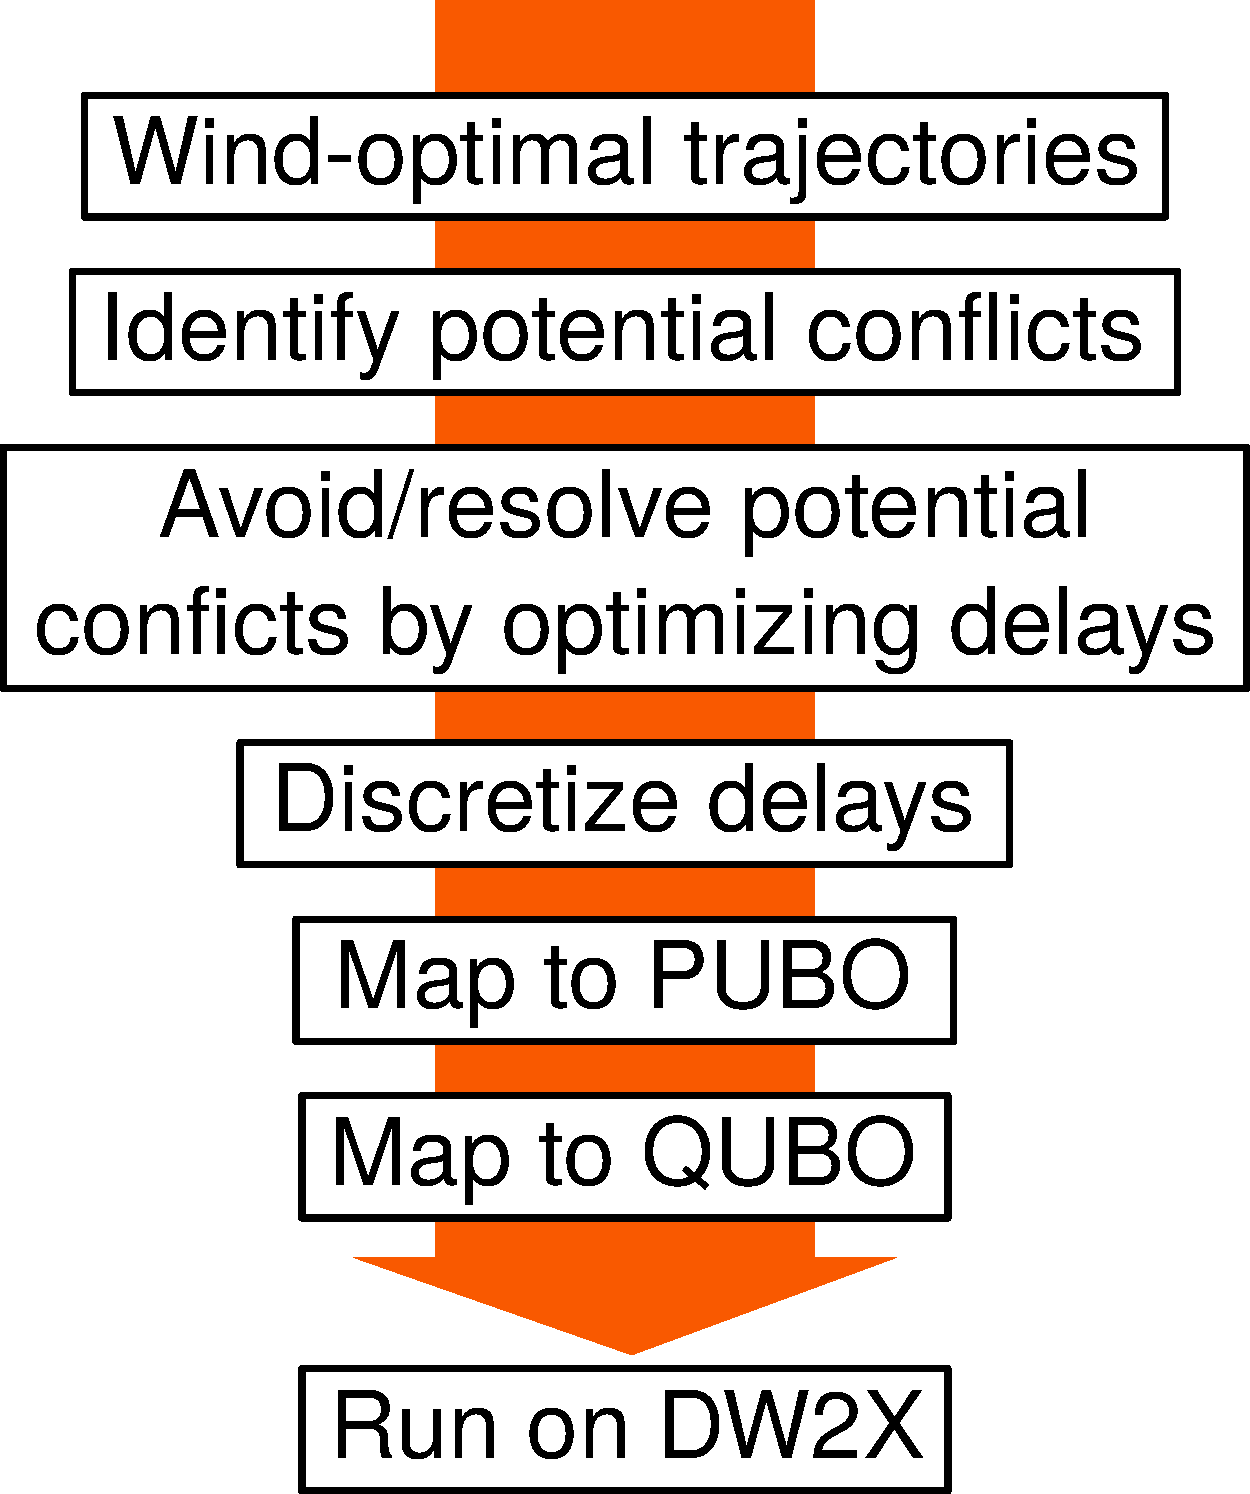
\includegraphics[width=0.35\textwidth]{scheme}
\caption{\label{fig:scheme}Flow diagram to map ATM problems into the \DW quantum chip.}
\end{wrapfigure}

\blindtext

\section*{Technical details}\label{sec:tech}

\blindtext

\section*{Assessment}\label{sec:ass}

\begin{table}[h!]\centering
	\begin{tabular}{|m{7cm}|m{7cm}|K{1.8cm}|}
		\rowcolor{gray!30}
		\hline
		\multicolumn{1}{|c|}{\textbf{Task/Milestone}} & \multicolumn{1}{c|}{\textbf{Performance Metric}} & \textbf{Expected completion}\\
		\hline
			Map the ATM problem to a suitable polynomial binary optimization problem (PUBO). & 
				Number of required logical qubits. Largest degree of the polynomial. Connectivity of the underlying coupling graph. & \checkmark\\
		\hline
			Map the ATM problem to a suitable quadratic binary optimization problem (QUBO). &
				Number of required logical qubits. Connectiviry of the underlying coupling graph. & \checkmark\\
		\hline
			Identify a set of benchmark ATM problems. & Hardness as a function of size. & 1 month\\
		\hline
			Analyze the results/performance of classical QUBO solvers on ATM problems. & 
				Assess the quality/variety of the solutions after discretization. Find the bottom line for classical computation. & 1.5 month\\
		\hline
			Find an embedding to map the ATM problem onto the Chimera architecture. & 
				Number of physical qubits for each logical qubit. Largest ATM problem embeddable on the current \DW chip. & 2 month\\
		\hline
			Compile the ATM benchmark ensemble for the \DW chip. & 
				Scaling of expected time to solution vs. size compared to classical code. Variety of different acceptable solutions. & 3 month\\
		\hline
			Outlook on different architectures and annealing strategies, hardware changes &
				Potential quantum enhancement. & 4 month\\
		\hline
	\end{tabular}\caption{\label{table:milestone}Breakdown of the project effort into milestones, including suggested performance metric and completion
		dates (check marks indicate completed tasks).}
\end{table}

\section*{Conclusion}\label{sec:conclusions}

%\bibliographystyle{apsrevtitle}
%\bibliography{refs.bib}

\end{document}
